\section*{Assignment 05: Governance and Data Policies}
\addcontentsline{toc}{section}{Assignment 05: Governance and Data Policies}

\subsection*{Onboarding and moderation architecture}
I combined \citet{Choudary2016}'s participation formula with \citet{Reillier2017}'s governance levers to draft the onboarding and moderation plan. Participation requires access, ability, and incentive. Access comes from institution issued logins for students and invitation codes for NGOs. Ability is supported by guided tours, contextual examples, and a first mission checklist. Incentive arrives through portfolio boosts for students and impact dashboards for organisations.

The onboarding journey unfolds in three concrete steps. First, a welcome screen previews sample projects and spells out expectations. Second, profile setup uses defaults for skills, availability, and preferred communication styles. Third, the first mission checklist unlocks only after users read the code of conduct and complete a practice task. Each step ends with a short micro survey so the team collects immediate feedback, reflecting Lecture~5's reminder to treat onboarding as an experiment \citep{Lecture05}.

Moderation follows a layered structure that maps to \citet{Choudary2016}'s categories of prevention, detection, and enforcement. Automated filters catch obvious spam. Community stewards, recruited from experienced students and NGO staff, can hide content temporarily and trigger review. A professional response team handles escalations within twenty four hours, relying on playbooks shaped with NGO advisors. Training includes de escalation scripts because course cases showed that many NGOs work with vulnerable communities, and mishandled communication can retraumatise participants \citep{Lecture11}. Quarterly tabletop drills test whether the process stays responsive.

\subsection*{Data policy and transparency}
Data collection sticks to the minimalism principle \citet{Zuboff2019} advocates. SkillSync only stores information needed for matching, payouts, and quality assurance: profile basics, project actions, satisfaction scores, and optional testimonials. Advanced analytics require explicit opt in during onboarding, and the default retention window is two years unless users request otherwise.

Transparency is implemented through a "data mirror" inside the product. Users can inspect every datapoint tied to their account, download it, or delete it unless a legal hold exists. Release notes summarise algorithm tweaks, moderation statistics, and incident reports every quarter. An internal ethics council meets monthly to vet new experiments. This council uses \citet{Reillier2017}'s governance canvas to evaluate whether changes shift power unfairly. External advisors from partner NGOs receive the same reports to keep legitimacy high \citep{Srnicek2017}.

Figure~\ref{fig:onboarding-flow} illustrates the four step carousel that anchors onboarding. Each panel includes plain language copy plus an indicator explaining why the step matters so users do not feel tricked. The design references the show not tell guidance from Lecture~5 on metrics and instrumentation \citep{Lecture05}.

\begin{figure}[H]
  \centering
  \makebox[\textwidth][c]{%
    \begin{minipage}[b]{0.42\textwidth}
      \centering
      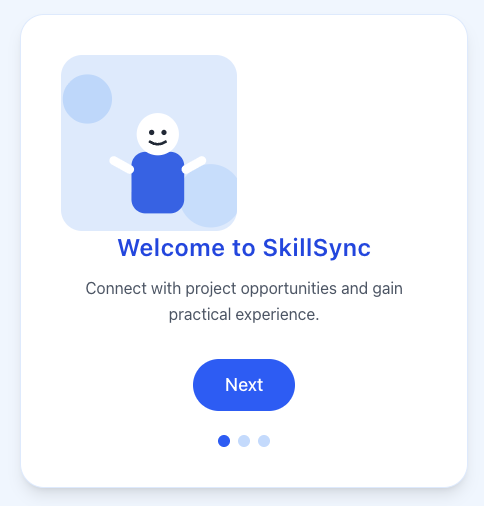
\includegraphics[width=\linewidth]{figures/Onboarding-1.png}\\[0.3em]
      
\includegraphics[width=\linewidth]{figures/Onboarding-2.png}
    \end{minipage}\hspace{1.5em}%
    \begin{minipage}[b]{0.42\textwidth}
      \centering
      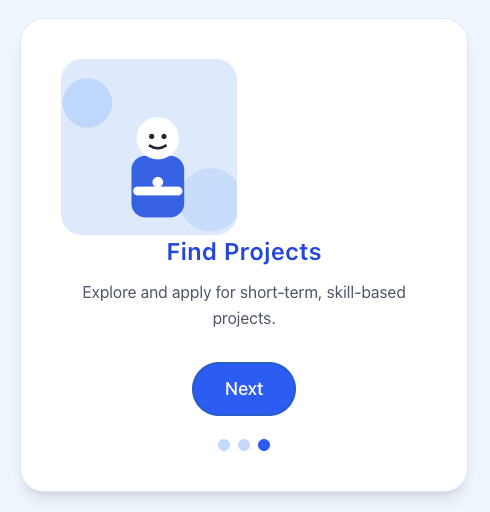
\includegraphics[width=\linewidth]{figures/Onboarding-3.png}\\[0.3em]
      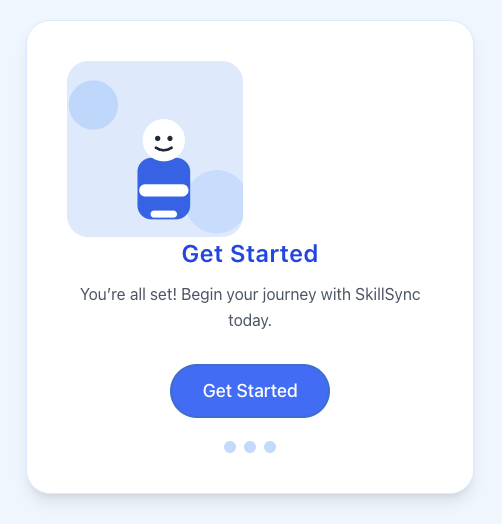
\includegraphics[width=\linewidth]{figures/Onboarding-4.png}
    \end{minipage}}
  \caption{Guided onboarding carousel with four step checklist.}
  \label{fig:onboarding-flow}
\end{figure}

Governance tooling appears in Figure~\ref{fig:admin-panel}. The administrator dashboard aggregates flagged content, dispute queues, and fairness metrics next to response time targets. Moderators can drill into case history, apply templated responses, escalate to legal counsel, and download evidence for quarterly reports. Those features map to the enforcement levers in \citet{Reillier2017} and keep accountability visible.

\begin{figure}[H]
  \centering
  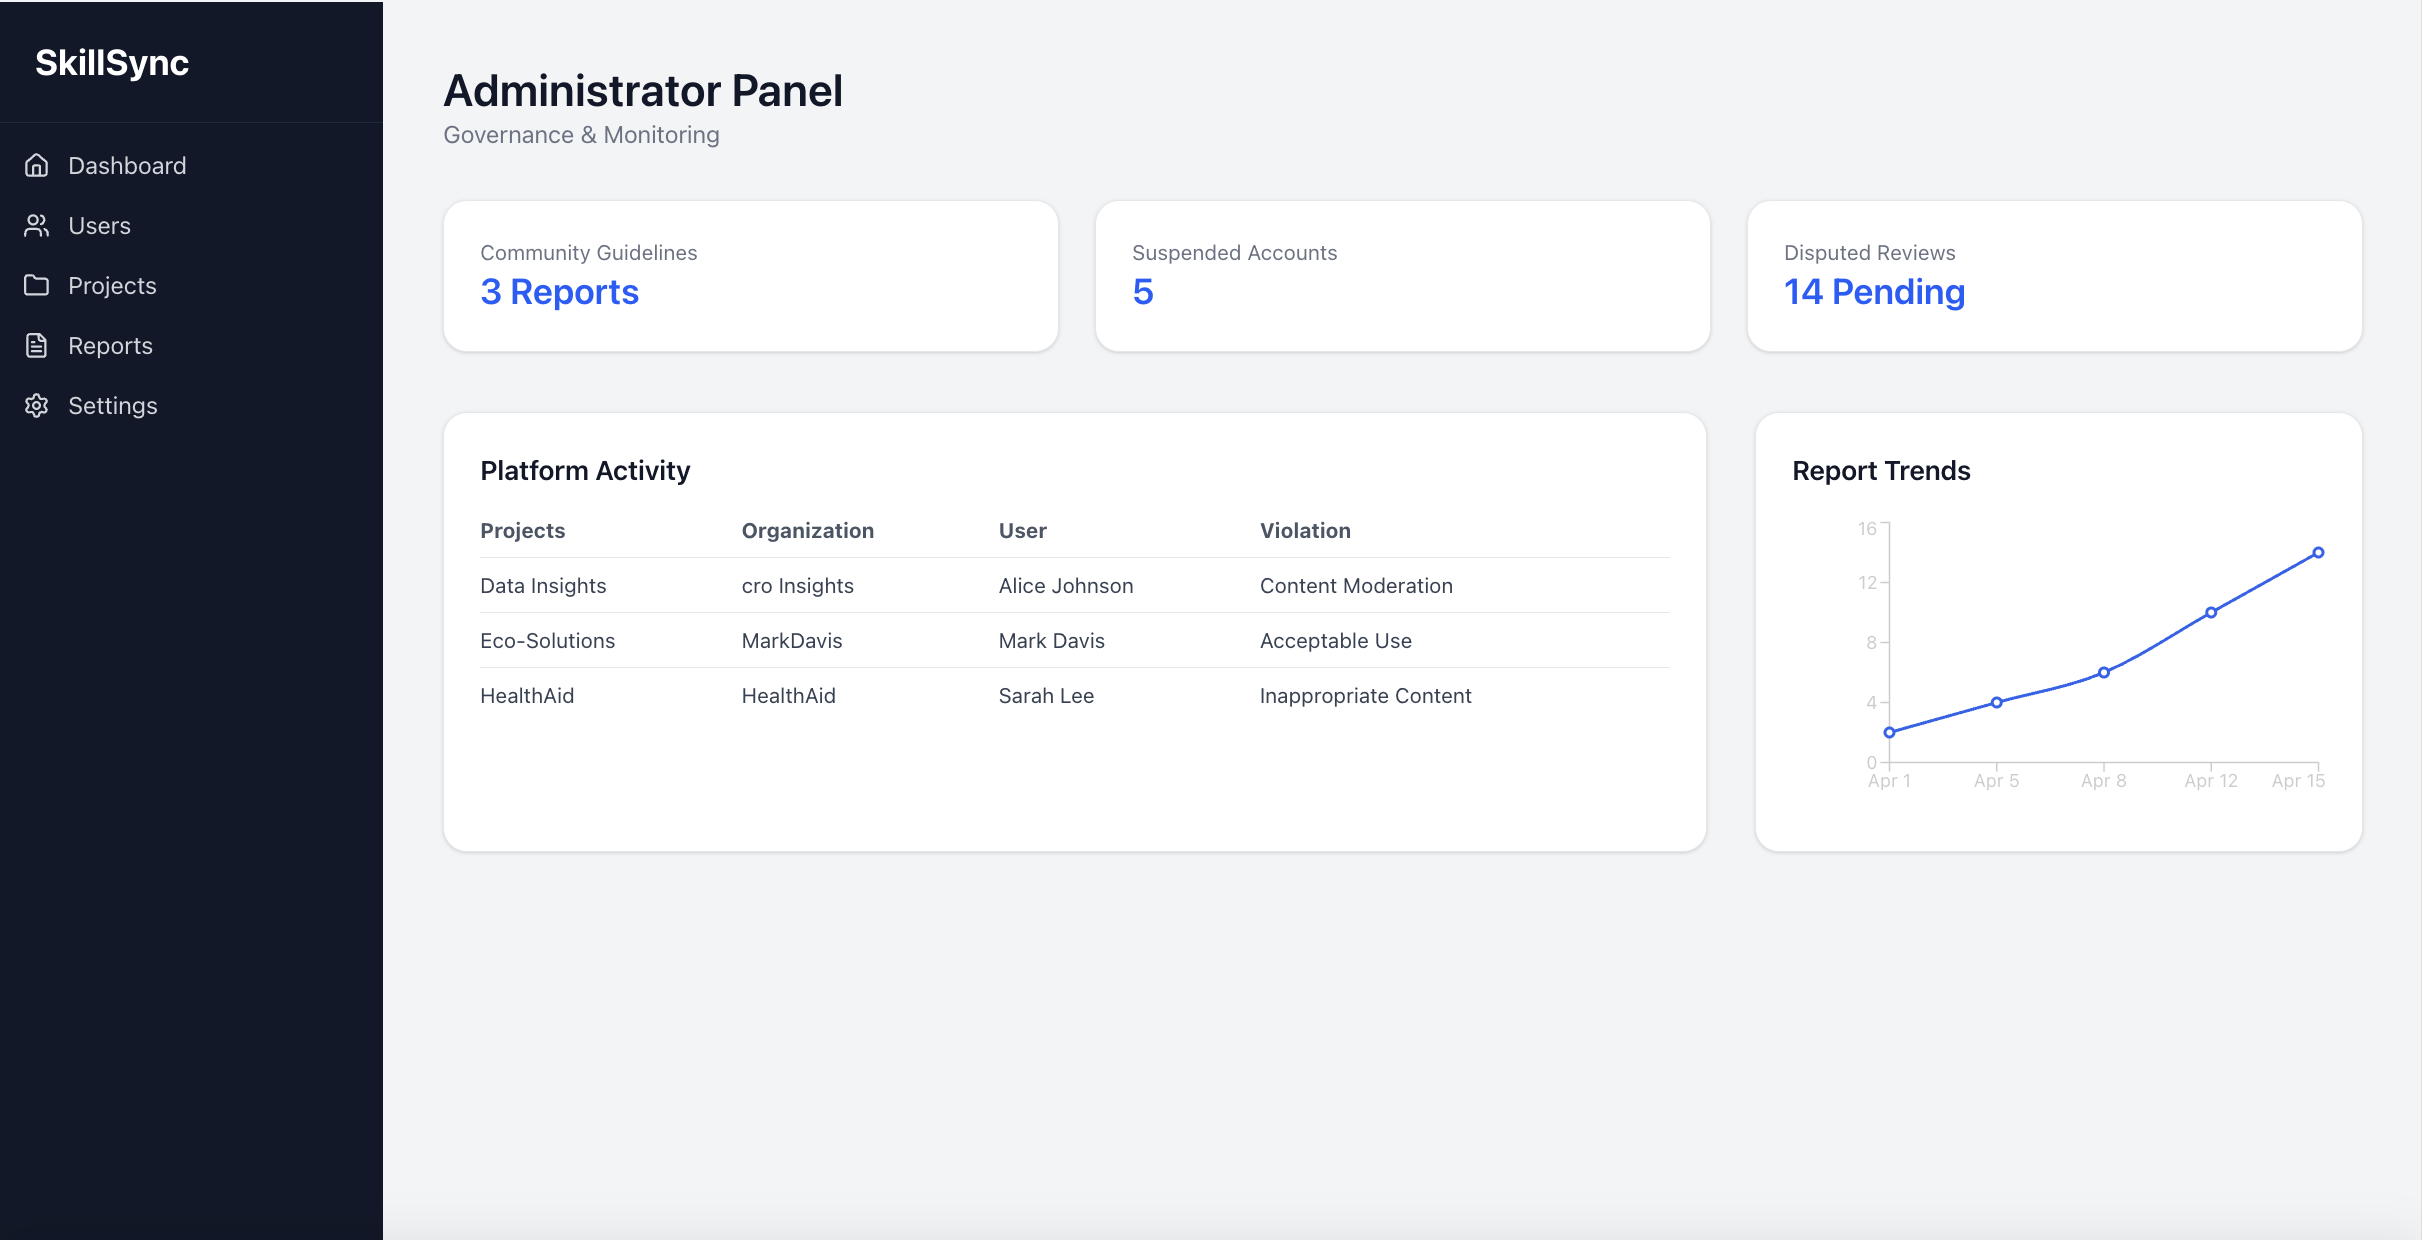
\includegraphics[width=0.85\linewidth]{figures/Organisation-Administratorpanel.png}
  \caption{Governance control room mock up with moderation and fairness metrics.}
  \label{fig:admin-panel}
\end{figure}

Finally, communication stays human. Automated nudges use friendly language and link to policy explanations. Moderators attend workshops led by partner NGOs to understand sensitive contexts. Quarterly community sessions let power users question the product team before major releases, honouring Lecture~11's call for legitimacy through dialogue \citep{Lecture11}.
